\documentclass[10pt]{article}
\usepackage[letterpaper,margin=0.75in]{geometry}
\usepackage{amsmath,amssymb,booktabs,array,graphicx,caption,float}
\captionsetup{font=small,labelfont=bf}
\setlength{\parskip}{3pt}\sloppy
\begin{document}
\begin{center}
{\Large\textbf{Exact line-of-sight tidal term for the Sedov--Taylor Center-of-Expansion model and its fit to the Migkas et al.\ (2020) cluster anisotropy}}\\[6pt]
{\small Worked sheet. Scripts: \texttt{figures/exact\_tidal\_core.py}, \texttt{exact\_termmatch.py}, \texttt{exact\_termmatch\_ext2.py}, \texttt{exact\_profile.py}, \texttt{exact\_termmatch\_plot.py}; sheet written by \texttt{papers/A\_equals\_fourier/make\_exact\_termmatch\_tex.py} from the result files.}
\end{center}

\section{Introduction}
Earlier sheets compared the Center-of-Expansion (CoE) model with the longitude dependence of the Migkas et al.\ cluster scaling-relation anisotropy $A(\ell)$. They used an analytic form of the tidal term expanded to first order in the ratio of the vision-shell radius to the distance from the CoE. That expansion was chosen only because it gives the sector-averaged harmonics in closed form. It is not a physical approximation, and the preferred solutions sit where the expansion parameter is close to one. In this sheet the line-of-sight tidal term is evaluated exactly, with no expansion. It is computed first for a point mass and then for an extended, decreasing density profile, averaged over the Migkas sectors, and projected numerically onto longitude harmonics. The harmonic-matching procedure is then repeated, and the distance ratio is treated as a continuous parameter that is fitted rather than sampled.

\section{Chris's variables and the model}
The model is written in Chris's variables. These are the vision-shell radius $r$ on which the sources sit, the observer's distance $D$ from the CoE, the density scale length $L$, the enclosed mass $M$ (the spreadsheet's $M/M_0$), the Galactic longitude $\ell_0$ and tilt $b_0$ of the CoE axis, the rotation phase $\varphi$ applied to the dipole, the phase $\varphi_2$ of the $2\ell$ term, and the harmonic amplitudes $\mathrm{Amp}_m$. The first-order analytic form used previously is
\begin{equation}
\frac{A}{A_{\rm all}}=N\Big[1+K\,(3\mu^2-1)+K\varepsilon\big(\tfrac92\mu-\tfrac{15}{2}\mu^3\big)\Big],
\label{eq:series}
\end{equation}
where $N$ is an overall normalisation, $K$ is the tidal strength defined in Sec.~\ref{sec:define}, $\varepsilon$ is the distance ratio defined there, and $\mu$ is the cosine of the angle between the line of sight and the CoE axis.

\section{Define parameters}\label{sec:define}
The compact parameters used below are
\begin{align}
\varepsilon&\equiv\frac{r}{D},\qquad x\equiv\frac{D}{L},\qquad \mu=\cos b\cos b_0\cos(\ell-\ell_0)+\sin b\sin b_0,\label{eq:def1}\\
\kappa&\equiv\frac{G\,M(<D)}{H^2D^3}=\frac{M(<D)}{2M_{\rm crit}(<D)},\qquad M_{\rm crit}(<D)=\frac{4\pi}{3}\rho_cD^3,\qquad K\equiv-\frac{u(D)}{H\,D}=\alpha\,\kappa,\label{eq:def2}
\end{align}
where $(\ell,b)$ is the direction of a source, $H$ is the Sedov--Taylor background expansion rate, $\rho_c$ is the critical density, $u(R)$ is the radial peculiar velocity at distance $R$ from the CoE, and $\alpha$ is the ratio between the tidal strength and the enclosed-mass parameter. In the earlier sheets $\alpha$ was left as an order-unity factor, and tables quoted $\alpha=1$. Here it is computed from the ideal-drag integration of the numerical code,
\begin{equation}
u(R,t_0)=-\int_{t_i}^{t_0}\exp\!\Big[-\!\int_{t'}^{t_0}H\,dt''\Big]\,\frac{G\,M\big(<R(t')\big)}{R(t')^2}\,dt',\qquad R(t')=R\,(t'/t_0)^{2/5},
\label{eq:drag}
\end{equation}
which for a point mass gives $\alpha=2/3$ analytically. Both conventions are tabulated.

\section{Exact line-of-sight tidal term}
With the CoE at the origin, the observer at $\vec x_o=D\hat x$ and a source at $\vec x_s=\vec x_o+r\hat n$, the fractional change of the observed expansion rate is
\begin{equation}
\frac{\delta H}{H}(\hat n)=\frac{\big[\vec u(\vec x_s)-\vec u(\vec x_o)\big]\cdot\hat n}{r\,H}=K\,\mathcal T(\mu,\varepsilon),\qquad
\mathcal T=\frac{1}{\varepsilon}\Big[\mu-f(\rho_s)\,\frac{\mu+\varepsilon}{\rho_s}\Big],\qquad \rho_s=\sqrt{1+2\varepsilon\mu+\varepsilon^2},
\label{eq:exact}
\end{equation}
where $f(\rho)=u(\rho D)/u(D)$ is the velocity shape and $\rho_s$ is the source's distance from the CoE in units of $D$. For a point mass the field is exactly inverse-square, so $f=\rho^{-2}$ and
\begin{equation}
\mathcal T_{\rm pm}=\frac{\mu-(\mu+\varepsilon)\,(1+2\varepsilon\mu+\varepsilon^2)^{-3/2}}{\varepsilon}
=(3\mu^2-1)+\varepsilon\big(\tfrac92\mu-\tfrac{15}{2}\mu^3\big)+O(\varepsilon^2).
\label{eq:pm}
\end{equation}
The expansion on the right is exactly Eq.~\eqref{eq:series} with $A/A_{\rm all}=N(1+K\mathcal T)$, so the normalisation and constant are unchanged, and the series is the small-$\varepsilon$ limit of the exact form. For the extended model the density is the pure exponential of the numerical code, $\rho\propto e^{-R/L}$ with $x$ free. The shape $f$ is obtained from Eq.~\eqref{eq:drag} with the enclosed mass computed by quadrature, and it tends to the point-mass shape as $x\to\infty$.

\section{Sector averaging and harmonic projection}
Each Migkas value is an average over a longitude sector of width $\Delta\ell$ centred at $\ell_c$, over all latitudes outside the Galactic-plane cut, with area weight $\cos b$ (Table~\ref{tab:setup}). Because the average is linear,
\begin{equation}
\Big\langle\frac{A}{A_{\rm all}}\Big\rangle(\ell_c)=N\big[1+K\tau_0\big]+NK\sum_{m\ge1}\tau_m\cos m(\ell_c-\ell_0),\qquad
\tau_m=W_m\,\frac{1}{\pi}\!\int_0^{2\pi}\!\bar{\mathcal T}(\psi)\cos m\psi\,d\psi,\qquad W_m=\frac{\sin(m\Delta\ell/2)}{m\Delta\ell/2},
\label{eq:tau}
\end{equation}
where $\bar{\mathcal T}(\psi)$ is the latitude average of $\mathcal T$ at longitude offset $\psi=\ell-\ell_0$, $W_m$ is the exact response of the sector boxcar, and $\tau_0$ is the mean with the $1/\pi$ replaced by $1/2\pi$. The sine terms vanish because $\mathcal T$ depends on $\psi$ only through $\cos\psi$. The first-order form gives $\tau_0=q_0$, $\tau_1=\varepsilon o_1$, $\tau_2=q_2$ and $\tau_3=\varepsilon o_3$, where $q_0,q_2,o_1,o_3$ are the closed-form latitude coefficients of the earlier sheets. The exact form also produces harmonics above $m=3$. The latitude integral uses Gauss--Legendre nodes and the longitude integral a uniform periodic grid; the numerical settings and checks are listed in Table~\ref{tab:setup}.


\begin{table}[!htb]\centering\small
\caption{Analysis settings and numerical checks.}\label{tab:setup}
\begin{tabular}{ll}\toprule
Quantity & Value\\\midrule
Vision-shell radius $r$ & $14.3$ Gpc\\
Sector width $\Delta\ell$; sector spacing; number of data points & $90^\circ$; $5^\circ$; $71$\\
Latitude cut; area weight & $|b|>20^\circ$; $\cos b$\\
CoE axis longitude $\ell_0$ (quadrupole peak of the data) & $14.96^\circ$\\
Quadrature (scans; convergence check) & $300\times2$ latitude nodes, $720$ longitudes; $800\times2$, $2880$\\
Harmonics retained in model curves & $m\le30$\\
Max.\ difference, harmonic route vs brute-force $72$-sector average & $1.2\times10^{-7}$\\
$\max|\mathcal T_{\rm pm}-\mathcal T_{\rm series}|/\varepsilon^2$ at $\varepsilon=0.1,\,0.01,\,0.001$ & 4.568, 4.051, 4.005\\
Point-mass $\alpha$: analytic; numerical (Euler) integration & $2/3$; $0.6603$\\\bottomrule
\end{tabular}
\end{table}


\section{Data harmonics and uncertainties}
The data are summarised by the least-squares Fourier fit to the digitised points,
\begin{equation}
A_{\rm fit}(\ell)=A_0+\sum_{m=1}^{3}A_m\cos m(\ell-\ell_m),
\label{eq:datafit}
\end{equation}
where $A_m$ and $\ell_m$ are the amplitude and peak longitude of harmonic $m$. Their uncertainties are propagated from the coefficient covariance in two ways. The adopted ``sector-correlated'' covariance accounts for the overlap of neighbouring sectors, which share a fraction $\max(0,1-|\ell_i-\ell_j|/\Delta\ell)$ of their clusters. The ``naive'' covariance treats all points as independent. Both are given in Table~\ref{tab:data}.

\begin{table}[!htb]\centering\small
\caption{Data harmonics of the Migkas $A(\ell)$ curve and their $1\sigma$ uncertainties.}\label{tab:data}
\begin{tabular}{lcccc}\toprule
 & $A_0$ & $A_1$ & $A_2$ & $A_3$\\\midrule
Amplitude & $0.9965$ & $0.0525$ & $0.0734$ & $0.0320$\\
Peak longitude $\ell_m$ & -- & $55.70^\circ$ & $14.96^\circ$ & $66.96^\circ$\\
$\sigma$, sector-correlated (adopted) & $0.0489$ & $0.0602$ & $0.0439$ & $0.0212$\\
$\sigma$, naive & $0.0115$ & $0.0156$ & $0.0160$ & $0.0157$\\\bottomrule
\end{tabular}
\end{table}

\section{Matching procedure}
Setting model and data amplitudes equal gives four equations,
\begin{equation}
N(1+K\tau_0)=A_0,\qquad NK|\tau_1|=A_1,\qquad NK|\tau_2|=A_2,\qquad NK|\tau_3|=A_3,
\label{eq:match}
\end{equation}
where every $\tau_m$ is a function of $(b_0,\varepsilon)$ for the point mass and of $(b_0,\varepsilon,x)$ for the extended density. With $\varepsilon$ free, the point-mass problem has four unknowns $(N,K,b_0,\varepsilon)$ and can be solved exactly. With $\varepsilon$ fixed it is overdetermined and is solved by least squares. Because $N$ appears only in the first equation, it is eliminated through $N=A_0-P\tau_0$ with $P\equiv NK$, and the objective is
\begin{equation}
\chi^2(b_0,\varepsilon\,[,x])=\min_P\sum_{m=1}^{3}\frac{\big(A_m-P|\tau_m|\big)^2}{\sigma_m^2},\qquad
P=\frac{\sum_m A_m|\tau_m|/\sigma_m^2}{\sum_m\tau_m^2/\sigma_m^2}.
\label{eq:chi2}
\end{equation}
The transforms are applied as before. The rotation sets the dipole peak to the data, $\phi_1=\ell_1-\ell^{(1)}_{\rm nat}$, where $\ell^{(1)}_{\rm nat}$ is $\ell_0$ for $\tau_1>0$ (``on-axis'' dipole) and $\ell_0+180^\circ$ for $\tau_1<0$ (``flipped''). The $2\ell$ phase $\phi_2$ sets the quadrupole peak to the data. The octupole and all higher harmonics keep their natural phases. The model curve compared with the points is then
\begin{equation}
A_{\rm mod}(\ell)=N(1+K\tau_0)+\sum_{m=1}^{2}NK|\tau_m|\cos m(\ell-\ell_m)+NK|\tau_3|\cos 3(\ell-\ell^{(3)}_{\rm nat})+\sum_{m\ge4}NK\tau_m\cos m(\ell-\ell_0),
\label{eq:curve}
\end{equation}
and in Chris's notation $\varphi=90^\circ-\ell_1$ and $\varphi_2=90^\circ-2\ell_2$. Two objectives are used when $D/r$ is fitted as a continuous parameter. The first is the amplitude $\chi^2$ of Eq.~\eqref{eq:chi2}. The second is the coefficient of determination $R^2$ of Eq.~\eqref{eq:curve} against the points, with $N$ and $P$ fitted linearly. Each is profiled over the remaining parameters,
\begin{equation}
\chi^2_{\rm prof}(D/r)=\min_{b_0\,[,x]}\chi^2,\qquad R^2_{\rm prof}(D/r)=\max_{N,P,b_0\,[,x]}R^2,\qquad 1<D/r\le6,
\label{eq:profile}
\end{equation}
and the intervals quoted are the ranges where $\chi^2_{\rm prof}$ lies within one and four of its minimum.


\section{Results}
\subsection{Exact versus first-order coefficients}
Table~\ref{tab:limit} checks the small-$\varepsilon$ limit. The exact coefficients converge to the first-order ones, and the residual falls as $\varepsilon^2$, as Eq.~\eqref{eq:pm} requires. Table~\ref{tab:ratio} and Fig.~\ref{fig:exact}a,b show that the two forms separate strongly when $D/r$ approaches one. The largest change is a suppression of the quadrupole and octupole coefficients when the CoE axis lies near the plane. When the tilt is closer to the free-solution value the changes are milder but still noticeable.

\begin{table}[!htb]\centering\small
\caption{Ratio of exact to first-order sector-averaged coefficients, $\tau_m^{\rm exact}/\tau_m^{\rm series}$, in the small-$\varepsilon$ limit.}\label{tab:limit}
\begin{tabular}{cccccc}\toprule
$b_0$ & $\varepsilon$ & monopole & dipole & quadrupole & octupole\\\midrule

$0.0^\circ$ & $0.3$ & $1.07735$ & $1.01754$ & $0.88730$ & $0.87626$\\
$0.0^\circ$ & $0.1$ & $1.00822$ & $1.00172$ & $0.98747$ & $0.98610$\\
$0.0^\circ$ & $0.03$ & $1.00074$ & $1.00015$ & $0.99887$ & $0.99875$\\
$0.0^\circ$ & $0.01$ & $1.00008$ & $1.00002$ & $0.99987$ & $0.99986$\\
$19.1^\circ$ & $0.3$ & $1.00360$ & $0.98728$ & $0.97176$ & $0.99426$\\
$19.1^\circ$ & $0.1$ & $1.00072$ & $0.99900$ & $0.99686$ & $0.99948$\\
$19.1^\circ$ & $0.03$ & $1.00007$ & $0.99991$ & $0.99972$ & $0.99995$\\
$19.1^\circ$ & $0.01$ & $1.00001$ & $0.99999$ & $0.99997$ & $0.99999$\\
$40.0^\circ$ & $0.3$ & $1.35290$ & $1.01567$ & $1.21287$ & $1.34015$\\
$40.0^\circ$ & $0.1$ & $1.03897$ & $1.00188$ & $1.02372$ & $1.03785$\\
$40.0^\circ$ & $0.03$ & $1.00350$ & $1.00017$ & $1.00214$ & $1.00341$\\
$40.0^\circ$ & $0.01$ & $1.00039$ & $1.00002$ & $1.00024$ & $1.00038$\\
\bottomrule
\end{tabular}
\end{table}

\begin{table}[!htb]\centering\small
\caption{Ratio of exact to first-order coefficients at finite distance ratio, for an in-plane axis and for a tilt near the free solution.}\label{tab:ratio}
\begin{tabular}{c cccc cccc}\toprule
 & \multicolumn{4}{c}{$b_0=0^\circ$} & \multicolumn{4}{c}{$b_0=19.1^\circ$}\\\cmidrule(lr){2-5}\cmidrule(lr){6-9}
$D/r$ & $\tau_0$ & $\tau_1$ & $\tau_2$ & $\tau_3$ & $\tau_0$ & $\tau_1$ & $\tau_2$ & $\tau_3$\\\midrule

$1.05$ & $1.808$ & $1.133$ & $-0.046$ & $-0.009$ & $1.139$ & $1.012$ & $0.643$ & $0.755$\\
$1.25$ & $1.654$ & $1.157$ & $0.198$ & $0.191$ & $0.921$ & $0.826$ & $0.826$ & $0.935$\\
$1.45$ & $1.482$ & $1.124$ & $0.397$ & $0.375$ & $0.952$ & $0.872$ & $0.866$ & $0.959$\\
$2.10$ & $1.209$ & $1.052$ & $0.715$ & $0.693$ & $0.996$ & $0.954$ & $0.931$ & $0.983$\\
$2.90$ & $1.104$ & $1.024$ & $0.851$ & $0.837$ & $1.003$ & $0.982$ & $0.963$ & $0.992$\\
$4.10$ & $1.050$ & $1.011$ & $0.926$ & $0.918$ & $1.003$ & $0.993$ & $0.981$ & $0.996$\\
$6.00$ & $1.023$ & $1.005$ & $0.965$ & $0.961$ & $1.002$ & $0.997$ & $0.991$ & $0.998$\\
\bottomrule
\end{tabular}
\end{table}


\subsection{Free distance ratio: exact solutions}
Solving Eq.~\eqref{eq:match} with all four unknowns free gives the roots in Table~\ref{tab:free}. The first-order form has one root with $D$ just above $r$ and one with $D<r$. With the exact point-mass form, both roots lie at $D>r$, so an exact four-harmonic match with the observer outside the vision shell exists. The roots were located on a $(b_0,\varepsilon)$ grid and refined, and they are unchanged on the finer quadrature. No other root exists in the scanned range. Close to $D/r=1$, however, the exact model also carries sizeable harmonics above the octupole, which the four equations do not constrain. These harmonics and the octupole phase offset lower $R^2$ at the exact roots.

\begin{table}[!htb]\centering\small
\caption{Exact four-harmonic solutions with free $D/r$ (amplitudes matched exactly, so all residuals vanish). The last column is the largest amplitude among the harmonics with $m\ge4$.}\label{tab:free}
\begin{tabular}{lcccccccc}\toprule
Model, branch & $D/r$ & $b_0$ & $N$ & $K$ & $\phi_1$ & $\delta_3$ & $R^2$ & max amp.\ $m\ge4$\\\midrule

First order, on-axis & $1.0075$ & $19.10^\circ$ & $1.0226$ & $0.1638$ & $+40.75^\circ$ & $-8.00^\circ$ & $0.897$ & $0$\\
First order, flipped & $0.9075$ & $31.66^\circ$ & $1.0047$ & $0.2055$ & $-139.25^\circ$ & $-8.00^\circ$ & $0.897$ & $0$\\
Exact point mass, on-axis & $1.1539$ & $18.87^\circ$ & $1.0297$ & $0.2122$ & $+40.75^\circ$ & $-8.00^\circ$ & $0.857$ & $0.0152$\\
Exact point mass, flipped & $1.1155$ & $40.33^\circ$ & $0.9760$ & $0.0989$ & $-139.25^\circ$ & $-8.00^\circ$ & $0.850$ & $0.0160$\\
\bottomrule
\end{tabular}
\end{table}


\subsection{Continuous fit of the distance ratio}
The profiles of Eq.~\eqref{eq:profile} are shown in Fig.~\ref{fig:profile}, and the best-fitting distance ratios with their intervals are collected in Table~\ref{tab:bestDr}. For the point mass the amplitude $\chi^2$ reaches zero at the exact roots of Table~\ref{tab:free}. It then rises slowly with $D/r$, and the rise is slower with the sector-correlated errors than with the naive ones. With either error model the four-unit threshold is not reached anywhere in the allowed range, because the octupole is itself only a marginal detection. For the extended density the $\chi^2$ is zero along a whole family of exact solutions, discussed below, so the extended fit does not select a unique $D/r$. The $R^2$ profile peaks slightly above $D/r=1$, falls steeply towards $D/r=1$ for the point mass because of the higher harmonics, and declines slowly at large $D/r$. The first-order profiles are included for comparison. The best-fit parameters are listed in Table~\ref{tab:bestpar} and translated into Chris's variables in Table~\ref{tab:chris}.

\begin{table}[!htb]\centering\small
\caption{Best-fit $D/r$ from the continuous profile fit, $1<D/r\le6$. For $\chi^2$ the best value is where the profile vanishes (an exact solution) or is smallest; the intervals are where $\Delta\chi^2\le1$ and $\le4$. ``1 (bound)'' means the interval extends to the constraint $D/r>1$.}\label{tab:bestDr}
\begin{tabular}{llcccc}\toprule
Model & Objective & best $D/r$ & min.\ $\chi^2$ or max.\ $R^2$ & $\Delta\chi^2\le1$ & $\Delta\chi^2\le4$\\\midrule

Exact point mass & $\chi^2$, sector-corr. & 1.115, 1.154 (roots) & $0.000$ & 1 (bound) -- 3.31 & 1 (bound) -- $>6$\\
Exact point mass & $\chi^2$, naive & 1.115, 1.154 (roots) & $0.000$ & 1 (bound) -- 2.11 & 1 (bound) -- $>6$\\
Exact point mass & $R^2$ (max) & 1.44 & $0.8979$ & -- & --\\
\midrule
Exact extended & $\chi^2$, sector-corr. & 1.01--1.15 (family) & $0.000$ & 1 (bound) -- 3.31 & 1 (bound) -- $>6$\\
Exact extended & $\chi^2$, naive & 1.01--1.14 (family) & $0.000$ & 1 (bound) -- 2.11 & 1 (bound) -- $>6$\\
Exact extended & $R^2$ (max) & 1.12 & $0.8980$ & -- & --\\
\midrule
First order & $\chi^2$, sector-corr. & 1.0075 (root) & $0.000$ & 1 (bound) -- 3.26 & 1 (bound) -- $>6$\\
First order & $\chi^2$, naive & 1.0075 (root) & $0.000$ & 1 (bound) -- 2.14 & 1 (bound) -- $>6$\\
First order & $R^2$ (max) & 1.12 & $0.8981$ & -- & --\\
\bottomrule
\end{tabular}
\end{table}


\begin{table}[!htb]\centering\small
\caption{Profile values at selected distance ratios (minimum $\chi^2$ and maximum $R^2$ over the remaining parameters, transforms included).}\label{tab:profile}
\begin{tabular}{c ccc ccc ccc}\toprule
 & \multicolumn{3}{c}{exact point mass} & \multicolumn{3}{c}{exact extended} & \multicolumn{3}{c}{first order}\\\cmidrule(lr){2-4}\cmidrule(lr){5-7}\cmidrule(lr){8-10}
$D/r$ & $\chi^2_{\rm corr}$ & $\chi^2_{\rm naive}$ & $R^2$ & $\chi^2_{\rm corr}$ & $\chi^2_{\rm naive}$ & $R^2$ & $\chi^2_{\rm corr}$ & $\chi^2_{\rm naive}$ & $R^2$\\\midrule

$1.05$ & $0.005$ & $0.016$ & $0.833$ & $0.000$ & $0.000$ & $0.898$ & $0.002$ & $0.005$ & $0.898$\\
$1.10$ & $0.000$ & $0.001$ & $0.860$ & $0.000$ & $0.000$ & $0.898$ & $0.009$ & $0.024$ & $0.898$\\
$1.15$ & $0.001$ & $0.004$ & $0.875$ & $0.000$ & $0.004$ & $0.898$ & $0.020$ & $0.051$ & $0.898$\\
$1.20$ & $0.003$ & $0.007$ & $0.885$ & $0.003$ & $0.007$ & $0.898$ & $0.034$ & $0.085$ & $0.898$\\
$1.30$ & $0.024$ & $0.062$ & $0.894$ & $0.024$ & $0.062$ & $0.898$ & $0.071$ & $0.170$ & $0.897$\\
$1.44$ & $0.080$ & $0.197$ & $0.898$ & $0.080$ & $0.197$ & $0.898$ & $0.134$ & $0.308$ & $0.895$\\
$1.50$ & $0.111$ & $0.266$ & $0.898$ & $0.111$ & $0.266$ & $0.898$ & $0.164$ & $0.370$ & $0.894$\\
$2.00$ & $0.409$ & $0.875$ & $0.887$ & $0.409$ & $0.875$ & $0.887$ & $0.419$ & $0.872$ & $0.884$\\
$2.50$ & $0.674$ & $1.361$ & $0.876$ & $0.674$ & $1.361$ & $0.876$ & $0.654$ & $1.491$ & $0.871$\\
$3.00$ & $0.878$ & $1.915$ & $0.863$ & $0.878$ & $1.820$ & $0.866$ & $0.887$ & $2.172$ & $0.858$\\
$4.00$ & $1.256$ & $2.617$ & $0.848$ & $1.256$ & $2.617$ & $0.848$ & $1.280$ & $2.685$ & $0.847$\\
$5.00$ & $1.554$ & $2.980$ & $0.840$ & $1.547$ & $2.980$ & $0.840$ & $1.571$ & $3.013$ & $0.839$\\
$6.00$ & $1.734$ & $3.223$ & $0.835$ & $1.734$ & $3.223$ & $0.835$ & $1.746$ & $3.239$ & $0.834$\\
\bottomrule
\end{tabular}
\end{table}


\begin{figure}[!t]\centering
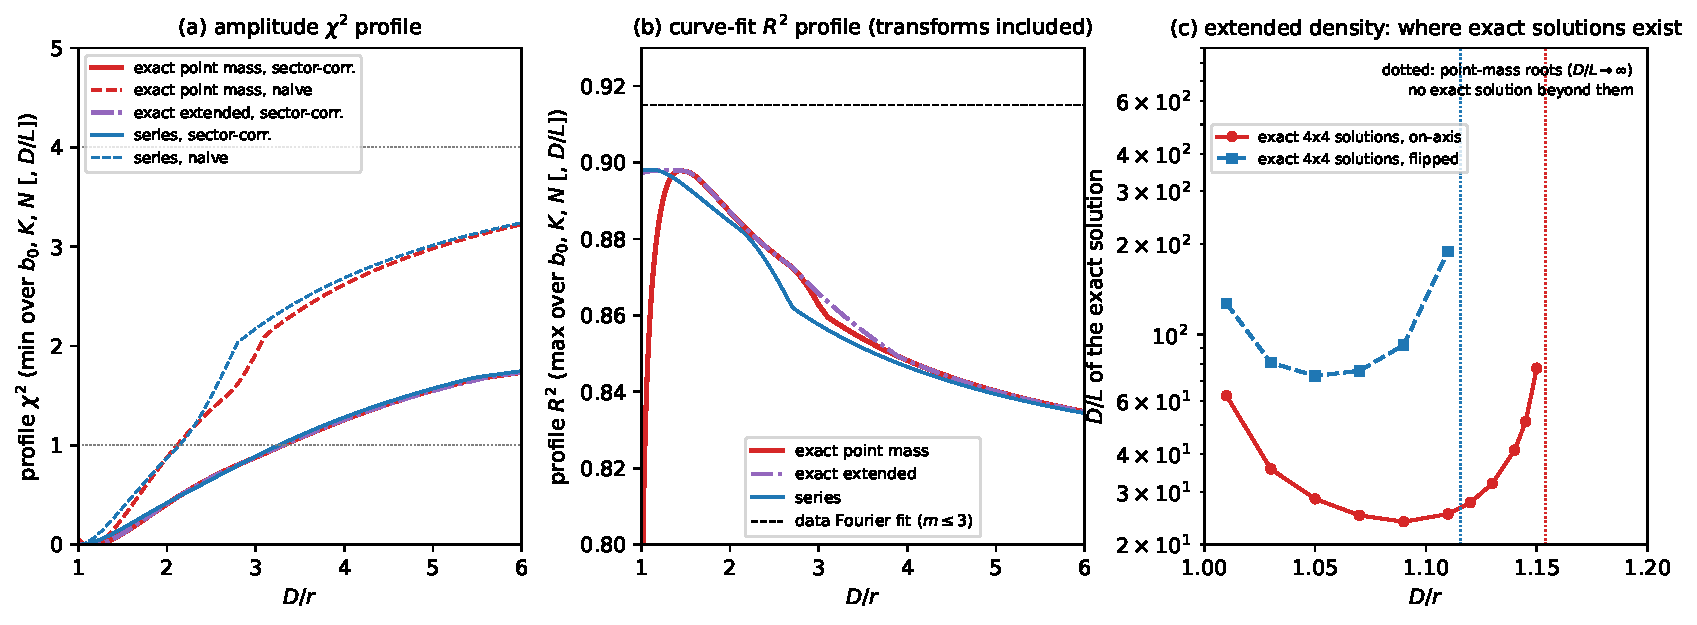
\includegraphics[width=\textwidth]{../../figures/exact_profile.pdf}
\caption{Continuous fit of the distance ratio. (a) Profile amplitude $\chi^2$ for the exact point mass, the exact extended density and the first-order form, with sector-correlated and naive errors; dotted lines mark $\Delta\chi^2=1$ and $4$. (b) Profile $R^2$ of the transformed curve against the digitised points; the dashed line is the data's own Fourier fit. (c) Exact four-harmonic solutions of the extended model: $D/L$ against $D/r$ for the two dipole branches; the vertical lines are the point-mass roots, which the extended family approaches as $D/L\to\infty$.}\label{fig:profile}
\end{figure}


\begin{table}[!htb]\centering\small
\caption{Best-fit parameters and predicted harmonics. Pulls are $(A_m^{\rm mod}-A_m)/\sigma_m$ with sector-correlated (c) and naive (n) errors; the $\chi^2$ roots match all amplitudes exactly.}\label{tab:bestpar}
\setlength{\tabcolsep}{3.5pt}
\begin{tabular}{lcccccccccc}\toprule
Solution & $D/r$ & $b_0$ & $D/L$ & $A_1$ & $A_2$ & $A_3$ & pull $A_3$ (c) & pull $A_3$ (n) & $\chi^2_{\rm corr}$ & $R^2$\\\midrule

Exact pm, $\chi^2$ root (on-axis) & $1.154$ & $18.87^\circ$ & $\infty$ & $0.0525$ & $0.0734$ & $0.0320$ & $-0.00$ & $-0.00$ & $0.000$ & $0.857$\\
Exact pm, $\chi^2$ root (flipped) & $1.115$ & $40.33^\circ$ & $\infty$ & $0.0525$ & $0.0734$ & $0.0320$ & $-0.00$ & $-0.00$ & $0.000$ & $0.850$\\
Exact pm, max $R^2$ & $1.441$ & $39.57^\circ$ & $\infty$ & $0.0528$ & $0.0749$ & $0.0243$ & $-0.36$ & $-0.49$ & $0.132$ & $0.898$\\
Exact extended, max $R^2$ & $1.120$ & $55.23^\circ$ & $12.6$ & $0.0527$ & $0.0748$ & $0.0246$ & $-0.35$ & $-0.47$ & $0.122$ & $0.898$\\
\bottomrule
\end{tabular}
\end{table}


\subsection{Reference rows at fixed distance ratio}
Table~\ref{tab:fixed} repeats the fixed-$D/r$ least-squares fits of the earlier sheet with the exact point-mass form, using the earlier weights. The dipole and quadrupole are still reproduced almost exactly, and the whole misfit remains in the octupole. From $D/r=2$ upward the exact and first-order octupole predictions agree closely, so the octupole shortfall found before is a property of the physics and not of the expansion. Only close to $D/r=1$ does the exact form raise the predicted octupole appreciably. The comparison is shown in Fig.~\ref{fig:exact}c.

\begin{table}[!htb]\centering\small
\caption{Fixed-$D/r$ least-squares fits with the exact point-mass form (weights from the naive errors, as in the earlier sheets; best branch). Pulls use the sector-correlated (c) and naive (n) errors. The last column is the first-order octupole at the same $D/r$.}\label{tab:fixed}
\setlength{\tabcolsep}{3.2pt}
\begin{tabular}{ccccccccccccc}\toprule
$D/r$ & branch & $b_0$ & $N$ & $K$ & $A_1$ & $A_2$ & $A_3$ & pulls $A_{1,2,3}$ (c) & pull $A_3$ (n) & $R^2$ & $A_3$ first order\\\midrule
data & & & & & $0.0525$ & $0.0734$ & $0.0320$ & & & $0.915$ & \\

$1.3$ & on-axis & $18.19^\circ$ & $1.0322$ & $0.2099$ & $0.0525$ & $0.0748$ & $0.0284$ & $-0.00,+0.03,-0.17$ & $-0.23$ & $0.891$ & $0.0259$\\
$2$ & on-axis & $13.65^\circ$ & $1.0403$ & $0.1970$ & $0.0524$ & $0.0769$ & $0.0177$ & $-0.00,+0.08,-0.67$ & $-0.91$ & $0.887$ & $0.0177$\\
$3$ & on-axis & $0.00^\circ$ & $1.0443$ & $0.1817$ & $0.0465$ & $0.0801$ & $0.0122$ & $-0.10,+0.15,-0.93$ & $-1.26$ & $0.863$ & $0.0091$\\
$4$ & flipped & $45.60^\circ$ & $0.9611$ & $0.2749$ & $0.0518$ & $0.0762$ & $0.0068$ & $-0.01,+0.07,-1.19$ & $-1.61$ & $0.848$ & $0.0064$\\
\bottomrule
\end{tabular}
\end{table}


\begin{figure}[!t]\centering
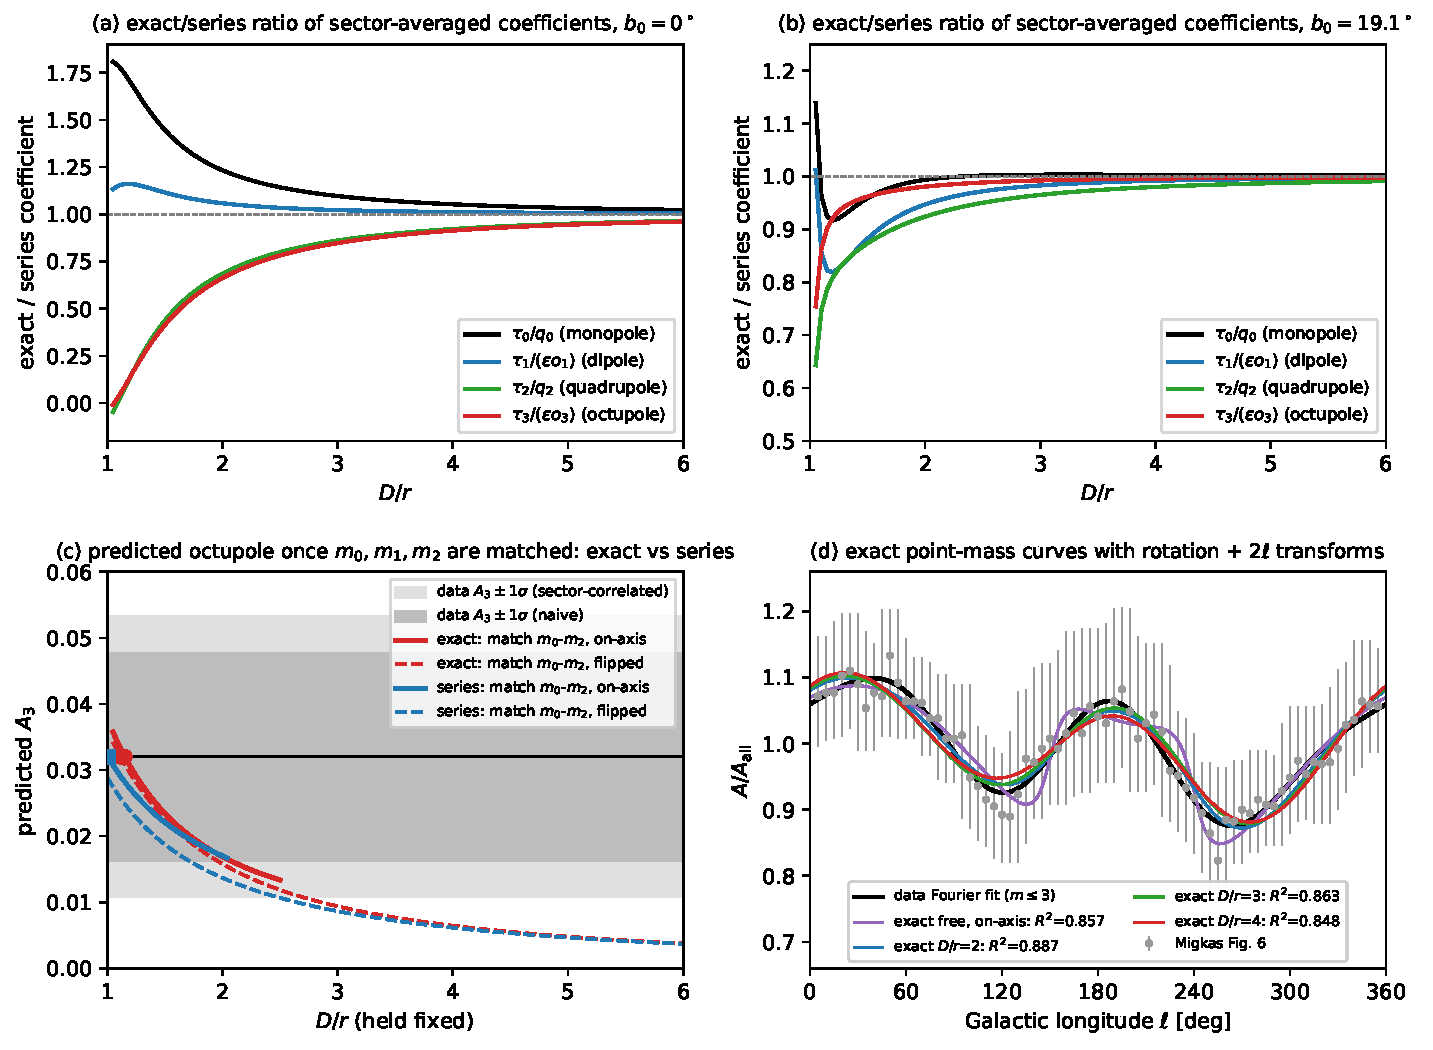
\includegraphics[width=\textwidth]{../../figures/exact_termmatch.pdf}
\caption{Exact versus first-order point-mass model. (a, b) Ratio of exact to first-order sector-averaged coefficients against $D/r$ for an in-plane axis and for a tilt near the free solution. (c) Octupole predicted after the monopole, dipole and quadrupole are matched exactly, for the exact form (red) and the first-order form (blue), on-axis (solid) and flipped (dashed) branches; grey bands show the data octupole with its sector-correlated and naive $1\sigma$ ranges; markers show the free-$D/r$ roots. (d) Digitised points, the data Fourier fit and exact point-mass curves with the transforms, for the exact on-axis root and the fixed-$D/r$ reference fits.}\label{fig:exact}
\end{figure}


\subsection{Extended density}
With the exponential density the extended mass restores a dipole that is larger relative to the quadrupole than for a point mass, and the scale length adds one unknown. At fixed $D/r$ the extended problem therefore has as many unknowns as equations. Exact solutions exist, but only on the family shown in Fig.~\ref{fig:profile}c and listed in Table~\ref{tab:ext}. That family runs from the point-mass roots, reached as $D/L\to\infty$, towards smaller $D/r$. No exact extended solution was found at larger distance ratios. There the least-squares optimum sits at the upper bound of the scale-length range, which is the point-mass limit, except for a narrow range where a finite scale length gives a marginally lower $\chi^2$. A finite scale length therefore does not relieve the octupole shortfall at large $D/r$. Along the exact family the curve-fit $R^2$ is lower than at the $R^2$-optimised solutions, again because of the higher harmonics and the octupole phase.

\begin{table}[!htb]\centering\small
\caption{Extended (exponential) density. Upper block: exact four-harmonic solutions ($N,K,b_0,D/L$ at fixed $D/r$). Lower block: least-squares optima where no exact solution exists ($D/L$ restricted to the scanned range, whose upper end is effectively a point mass).}\label{tab:ext}
\begin{tabular}{lcccccccc}\toprule
Type & $D/r$ & branch & $b_0$ & $D/L$ & $K$ & $\alpha$ & $A_3$ & $R^2$\\\midrule

exact & $1.01$ & flipped & $79.27^\circ$ & $126.9$ & $0.3035$ & $0.660$ & $0.0320$ & $0.854$\\
exact & $1.05$ & flipped & $61.45^\circ$ & $72.8$ & $0.1524$ & $0.659$ & $0.0320$ & $0.852$\\
exact & $1.09$ & flipped & $47.83^\circ$ & $92.3$ & $0.1123$ & $0.660$ & $0.0320$ & $0.851$\\
exact & $1.11$ & flipped & $41.83^\circ$ & $189.5$ & $0.1012$ & $0.660$ & $0.0320$ & $0.851$\\
exact & $1.01$ & on-axis & $77.68^\circ$ & $62.6$ & $0.6315$ & $0.658$ & $0.0320$ & $0.873$\\
exact & $1.05$ & on-axis & $53.99^\circ$ & $28.4$ & $0.3318$ & $0.642$ & $0.0320$ & $0.868$\\
exact & $1.09$ & on-axis & $34.55^\circ$ & $23.8$ & $0.2492$ & $0.634$ & $0.0320$ & $0.864$\\
exact & $1.11$ & on-axis & $28.03^\circ$ & $25.3$ & $0.2322$ & $0.637$ & $0.0320$ & $0.861$\\
exact & $1.13$ & on-axis & $23.25^\circ$ & $31.9$ & $0.2214$ & $0.646$ & $0.0320$ & $0.859$\\
exact & $1.15$ & on-axis & $19.57^\circ$ & $77.3$ & $0.2135$ & $0.659$ & $0.0320$ & $0.857$\\
\midrule
LSQ & $1.3$ & on-axis & $18.23^\circ$ & $200.0$ & $0.2100$ & $0.660$ & $0.0283$ & $0.891$\\
LSQ & $1.5$ & on-axis & $17.24^\circ$ & $200.0$ & $0.2068$ & $0.660$ & $0.0243$ & $0.898$\\
LSQ & $2$ & on-axis & $13.65^\circ$ & $200.0$ & $0.1969$ & $0.660$ & $0.0177$ & $0.887$\\
LSQ & $3$ & on-axis & $0.00^\circ$ & $17.6$ & $0.1849$ & $0.615$ & $0.0114$ & $0.866$\\
LSQ & $4$ & flipped & $45.59^\circ$ & $200.0$ & $0.2749$ & $0.660$ & $0.0068$ & $0.848$\\
LSQ & $6$ & flipped & $50.59^\circ$ & $200.0$ & $0.3681$ & $0.660$ & $0.0039$ & $0.835$\\
\bottomrule
\end{tabular}
\end{table}


\section{Translation to Chris's variables}
The fitted parameters are translated back with
\begin{equation}
D=r\,(D/r),\qquad \frac{M(<D)}{M_{\rm crit}}=2\kappa=\frac{2K}{\alpha},\qquad L=\frac{D}{x},\qquad \varphi=90^\circ-\ell_1,\qquad \varphi_2=90^\circ-2\ell_2,
\label{eq:chris}
\end{equation}
where the mass ratio is given both for $\alpha=1$ (the convention of the earlier sheets) and for the ideal-drag value of Eq.~\eqref{eq:drag}. Because the transforms place the dipole and quadrupole peaks on the data, $\varphi$ and $\varphi_2$ are the same for every solution. The results are in Table~\ref{tab:chris}.

\begin{table}[!htb]\centering\small
\caption{Best-fit solutions and fixed-$D/r$ reference fits in Chris's variables ($r=14.3$ Gpc). For all rows $\ell_0=14.96^\circ$, $\varphi=34.30^\circ$ and $\varphi_2=60.08^\circ$.}\label{tab:chris}
\setlength{\tabcolsep}{3.3pt}
\begin{tabular}{lccccccccc}\toprule
Solution & $D/r$ & $D$ [Gpc] & $D$ [Gly] & $K$ & $\frac{M}{M_{\rm crit}}$ ($\alpha{=}1$) & $\frac{M}{M_{\rm crit}}$ (drag) & $b_0$ & $\phi_1$ & $L$ [Gpc]\\\midrule

Exact pm, $\chi^2$ root (on-axis) & $1.154$ & $16.50$ & $53.8$ & $0.2122$ & $0.424$ & $0.643$ & $18.87^\circ$ & $+40.75^\circ$ & --\\
Exact pm, $\chi^2$ root (flipped) & $1.115$ & $15.95$ & $52.0$ & $0.0989$ & $0.198$ & $0.300$ & $40.33^\circ$ & $-139.25^\circ$ & --\\
Exact pm, max $R^2$ & $1.441$ & $20.60$ & $67.2$ & $0.1277$ & $0.255$ & $0.387$ & $39.57^\circ$ & $-139.25^\circ$ & --\\
Exact extended, max $R^2$ & $1.120$ & $16.02$ & $52.2$ & $0.3984$ & $0.797$ & $1.370$ & $55.23^\circ$ & $+40.75^\circ$ & $1.266$\\
Exact pm, fixed $D/r=2$ & $2.000$ & $28.60$ & $93.3$ & $0.1970$ & $0.394$ & $0.597$ & $13.65^\circ$ & $+40.75^\circ$ & --\\
Exact pm, fixed $D/r=3$ & $3.000$ & $42.90$ & $139.9$ & $0.1817$ & $0.363$ & $0.550$ & $0.00^\circ$ & $+40.75^\circ$ & --\\
Exact pm, fixed $D/r=4$ & $4.000$ & $57.20$ & $186.6$ & $0.2749$ & $0.550$ & $0.833$ & $45.60^\circ$ & $-139.25^\circ$ & --\\
\bottomrule
\end{tabular}
\end{table}

\section{Conclusions}
Evaluating the tidal term exactly changes the harmonic coefficients substantially only when the observer is within a few vision-shell radii of the CoE (Table~\ref{tab:ratio}). Farther out, the first-order form was an adequate description. With four unknowns, an exact match of all four measured harmonics now exists with the observer outside the vision shell, on both dipole branches (Table~\ref{tab:free}). The preferred distance ratio therefore moves from essentially unity to slightly above it, but it stays close to one.

Treating $D/r$ as a continuous parameter does not tighten this much (Table~\ref{tab:bestDr}, Fig.~\ref{fig:profile}). The amplitude $\chi^2$ grows only slowly with distance, and even the four-unit threshold is not crossed within the allowed range, so the octupole alone cannot exclude large distance ratios even at the level of the wider interval. The curve-fit $R^2$ is highest slightly above unity and degrades gradually, and the differences are small compared with what overlapping sectors can support.

The octupole tension at fixed $D/r\ge2$ is essentially the same with the exact form as with the series (Table~\ref{tab:fixed}, Fig.~\ref{fig:exact}c). It is not an artefact of the expansion. An extended exponential density does not rescue large distance ratios either: its extra freedom produces exact solutions only between the point-mass roots and $D/r=1$ (Table~\ref{tab:ext}).

Close to $D/r=1$ the exact model develops harmonics above the octupole, which the four-harmonic matching ignores. As a result, the exactly matching solutions have a lower $R^2$ than the $R^2$-optimised ones. Caveats carried over from the earlier sheets remain. The rotation and $2\ell$ phases are free rather than predicted. The error model assumes uniform clusters and statistical, overlap-correlated error bars read from a digitised figure. The sector averages assume a uniform sky outside the plane cut. Only a single-exponential density family was tried for the extended mass.
\end{document}
